\documentclass[12pt,a4paper]{article}

%%%%%%%%%%%%%%%%%%%%%%%%% packages %%%%%%%%%%%%%%%%%%%%%%%%
\usepackage{amsmath}
\usepackage{amssymb}
\usepackage{amsthm}
\usepackage{amsfonts}
\usepackage{graphicx}
\usepackage[utf8]{inputenc}
\usepackage[english]{babel}
\usepackage[all]{xy}
\usepackage{float}
\usepackage{tikz}
\usepackage{verbatim}
\usepackage[left=2cm,right=2cm,top=2cm,bottom=2cm]{geometry}
\usepackage{hyperref}
\usepackage{caption}
\usepackage{subcaption}
\usepackage{psfrag}
\usepackage{natbib}
%\bibliographystyle{abbrvnat}
\usepackage{booktabs}  
\usepackage[T1]{fontenc}    % use 8-bit T1 fonts
\usepackage{url} 


%%%%%%%%%%%%%%%%%%%%% students data %%%%%%%%%%%%%%%%%%%%%%%%
\newcommand{\student}{Brian KYANJO }
\newcommand{\course}{Dr. Jodi Mead, Michal Kopera, and Dylan Mikesell}
\newcommand{\assignment}{ Prof. Donna Calhoun}

%%%%%%%%%%%%%%%%%%% using theorem style %%%%%%%%%%%%%%%%%%%%
\newtheorem{thm}{Theorem}
\newtheorem{lem}[thm]{Lemma}
\newtheorem{defn}[thm]{Definition}
\newtheorem{definition}{Definition}[section] 
\newtheorem{theorem}{Theorem}
\newtheorem{exa}[thm]{Example}
\newtheorem{rem}[thm]{Remark}
\newtheorem{coro}[thm]{Corollary}
\newtheorem{quest}{Question}[section]

%%%%%%%%%%%%%%  Shortcut for usual set of numbers  %%%%%%%%%%%

\newcommand{\N}{\mathbb{N}}
\newcommand{\Z}{\mathbb{Z}}
\newcommand{\Q}{\mathbb{Q}}
\newcommand{\R}{\mathbb{R}}
\newcommand{\C}{\mathbb{C}}

%%%%%%%%%%%%%%%%%%%%%%%%%%%%%%%%%%%%%%%%%%%%%%%%%%%%%%%555
\begin{document}
	
	%%%%%%%%%%%%%%%%%%%%%%% title page %%%%%%%%%%%%%%%%%%%%%%%%%%
	\thispagestyle{empty}
	\begin{center}
		\textbf{A Riemann Solver for Wet/Dry Interfaces in Geoclaw \\[0.5cm]
			Synthesis Paper}
		\vspace{.2cm}
	\end{center}
	
	%%%%%%%%%%%%%%%%%%%%% assignment information %%%%%%%%%%%%%%%%
	\noindent
	\rule{17cm}{0.2cm}\\[0.3cm]
	Name: \student \hfill Supervisor: \assignment\\[0.1cm]
	Committee: \course \hfill Date: \today\\
	\rule{17cm}{0.05cm}
	\vspace{.2cm}
	
	\section{Introduction}
	A Riemann Problem is a specific intial value problem  (Cauchy) of a partial differential equation (PDE) that consists of conservation equations combined with piecewise constant intial data which has a single discontinuity in the domain of interest as shown in equation\eqref{rp1}. 
	\begin{eqnarray}
		q_{t} + A q_{x}& =& 0
		\label{rp0}\\
		q(x,0)& =& \begin{cases}
			q_{L}, & \text{if \, $x \le 0,$}\\
			q_{R},& \text{if \, $x > 0,$}\\
			
		\end{cases}  
		\label{rp1}     
	\end{eqnarray}
	
	
	\noindent where $q_{R}$ and $q_{L}$ are two piecewise constant states separated by a discontinuity. Applying method of characteristics to the initial value problem (IVP) gives  equation \eqref{rp2} of the trajectory characteristic curve.
	
	\begin{equation}
		x = x_{o} + at 
		\label{rp2}
	\end{equation}
	
	
	\noindent Equation \eqref{rp2} is used to obtain the exact solution of the Riemann problem (equatio \eqref{rp3})
	\begin{equation}
		q(x,t)  = \begin{cases}
			q_{l}, & \text{if \, $x - at \le 0,$}\\
			q_{r},& \text{if \, $x - at > 0,$}\\
			
		\end{cases}    
		\label{rp3}   
	\end{equation}
	
		\section{Shallow Water Equations (SWE)}
	The SWE are a system of hyperbolic or parabolic (for viscous shear) PDEs governing the flow below a pressure surface in a fluid. They arise from the Navier-stokes equations and can be used to model a fluid in a channel of unit width, taking the vertical velocity negilible, and horizontal velocity roughly constant throughout any cross section of the channel \cite{ge:2008}.  \\
	
	\noindent Consider a small-amplitude waves in a fluid that is shallow relative to its wavelength. The conservation of momentum equation is written in terms of pressure, $p(x,t) = \frac{1}{2}\rho gh^{2}$, and the height field $h(x,t)$ ($m$), which breaks down into two equations \eqref{p1} and \eqref{p2}.
	
	\begin{eqnarray}
		h_{t} + (uh)_x &=& 0
		\label{p1} \\
		(hu)_t + \left(hu^{2} + \frac{1}{2}gh^{2} \right)_x &=& 0
		\label{p2}
	\end{eqnarray}	
	
	\noindent where $hu$ measures the flow rate of water past a point,  $\rho$ ($kg/m^3$) is the constant density of the incompressible fluid, and $u(x,t)$ ($m/s$) is the horizontal velocity.\\
	
	\noindent The variation of $h$ and $hu$ at each interface in both space and time leads the waves in the Riemann problem to move at different speeds creating discountinouities (shocks) or changing regions (rarefactions).  At $x = 0$ and $t = 0$,   the discountinuity is located between the left and right state, so the solution at the left ($q_{l}$)and right($q_{r}$) states are given by: 
	\begin{equation}
		q_{l} = \begin{bmatrix}
	h_{l} \\( hu)_{l}
		\end{bmatrix}  \quad \text{and} \quad q_{r} = \begin{bmatrix}
		h_{r} \\( hu)_{r}
	\end{bmatrix} 
	\end{equation}
	
	\noindent As $x$ and $t$ increases, a middle state called the intemediate state($q_{m}$), is generated, the determination of this state characterises the Riemann problem and how it connects to other states via waves in each respective characteristic family\cite{ba-le-mi-ro:2003}.  This can only hold if the connection wave speeds satisfy the Lax entropy condition. Figure \ref{fig:x-tplane} shows a wave combination of a centered rarefaction  and shock wave from the first and second characteristic family respectively.
	  
	\begin{figure}[H]
		\centering
		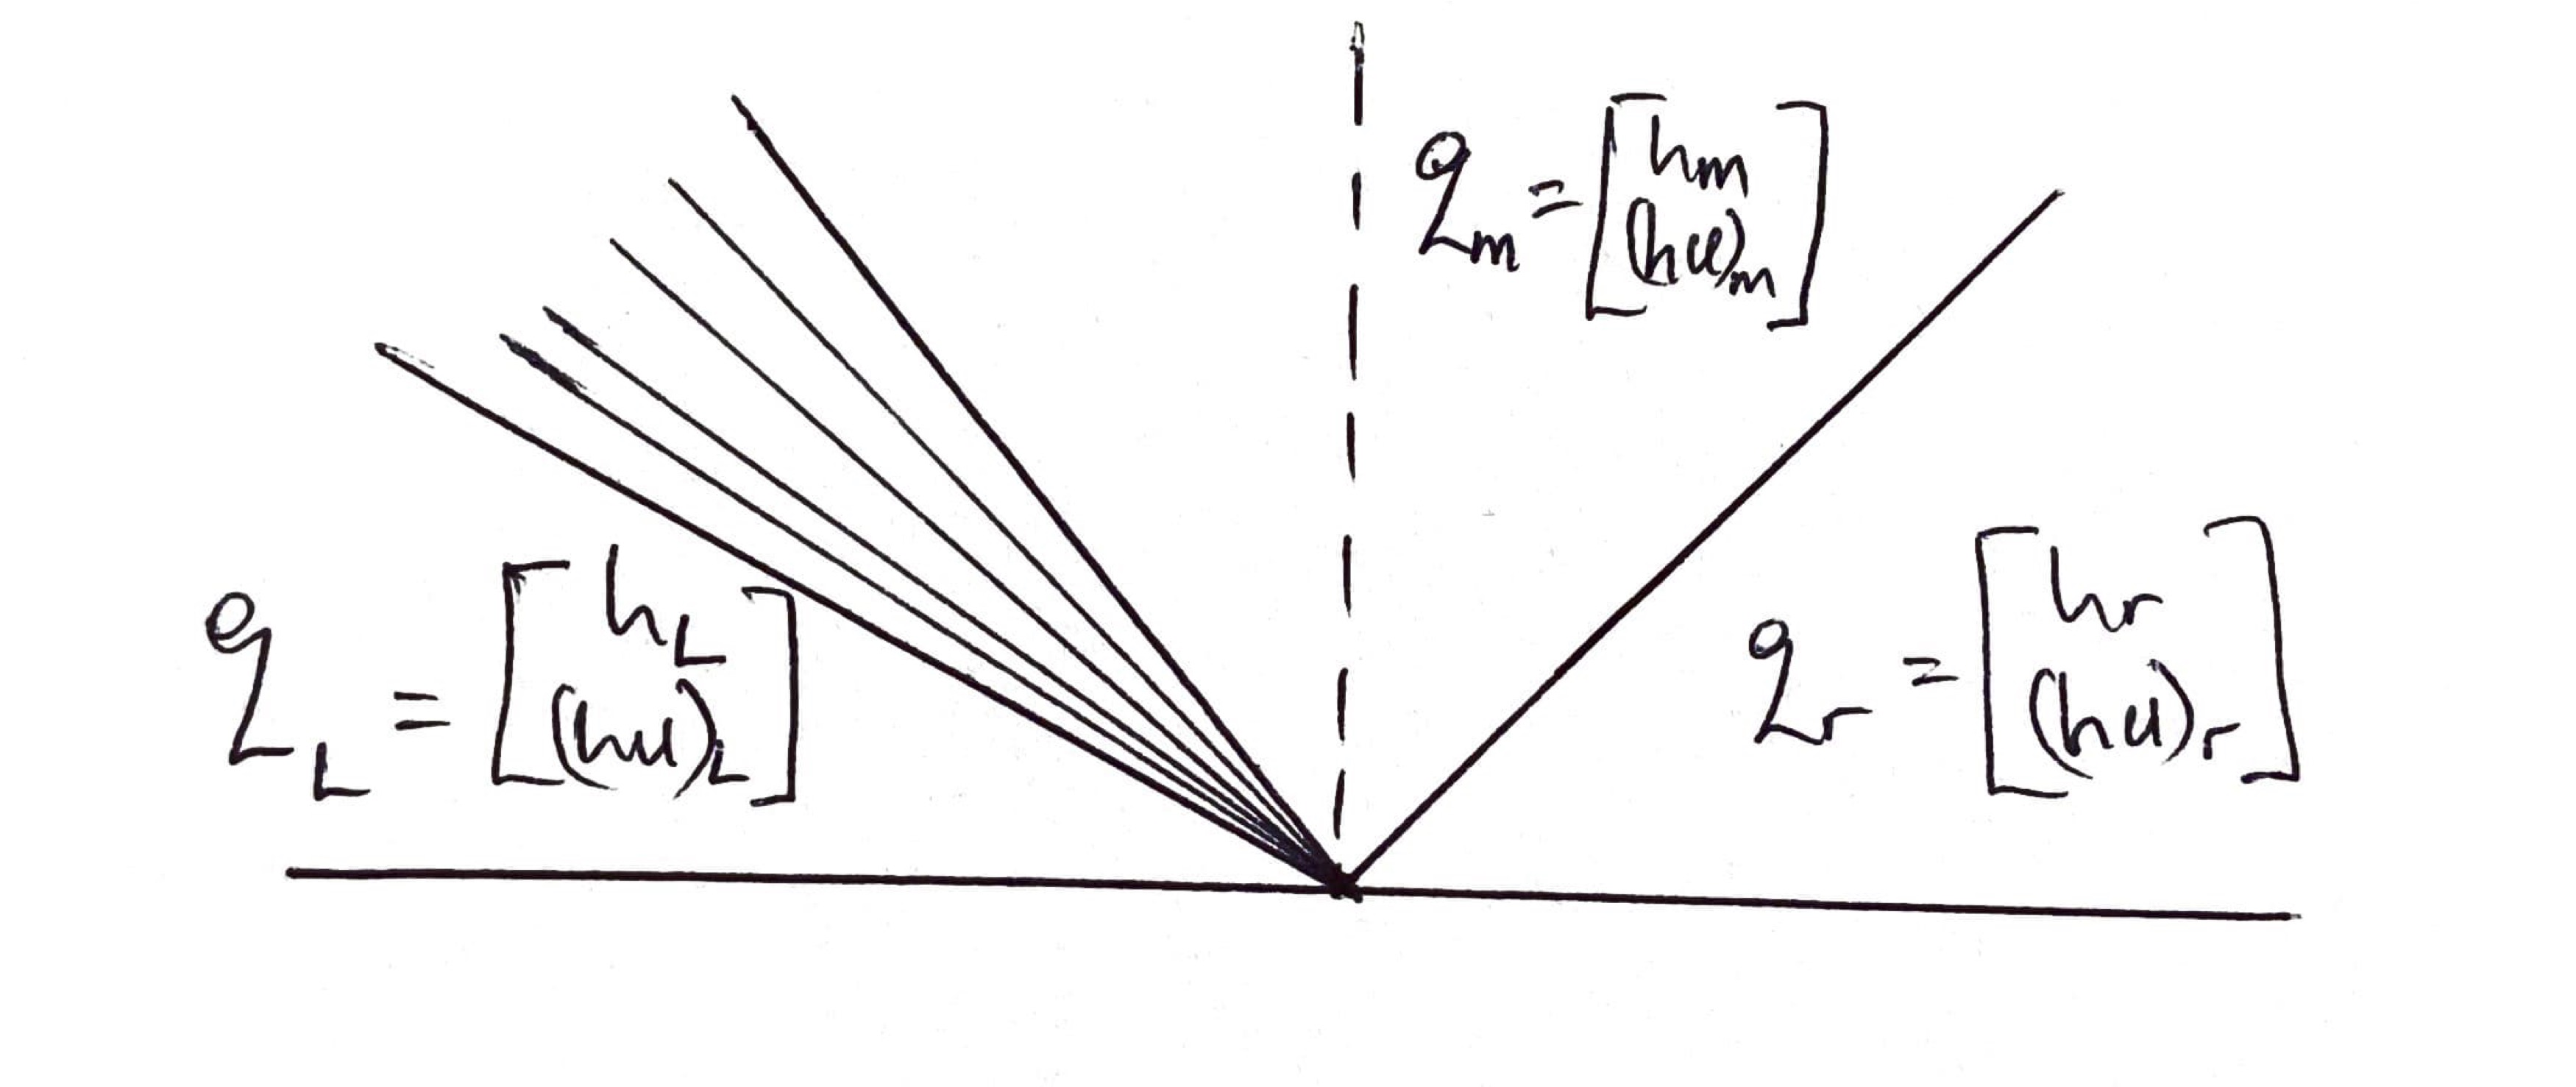
\includegraphics[width=0.5\linewidth]{images/x-t_plane}
		\caption{ x-t plane showing the connection of states, 1-rarefaction fan, and the 2-shock.}
		\label{fig:x-tplane}
	\end{figure}
	
	 \noindent The intermediate state is obtained by solving the Riemann problem using the exact or  approximate method. Although approximate methods are widely used due to their cheap computational cost compared to the exact solvers.
	
	
	\subsection{Exact Riemann Solver for SWE}
	\noindent The non linear equation is solved at each cell interface for each time step. The shock speed, $s(t)$,  from the shock wave as the solution emerges is determined from the Rankine-Hugoniot jump condition given by equation \eqref{e1}  which must be satisfied across any shock wave.
	\begin{equation}
		s(q_{r} - q_{l}) = f(q_{r}) - f(q_{l})
		\label{e1}
	\end{equation}
	
	\noindent where $f$ is the flux function. By applying this condition ( equation \eqref{e1}) to shallow water equations: \eqref{p1} and \eqref{p2}) creates a system of two equations that must be satisfied simultaneously. This system is used to derive expression for the Hugoniot Loci which we are used together with the intergral curves (equation \eqref{e2}) to obtain the intermediate state $q_{m}$. \\
	
	\noindent As an example, consider a known problem(dam break) with a 1-rarefaction and a 2-shock leading to a system of equations: \eqref{e2} and \eqref{e3} that are equated  to solve a resulting non linear equation for $u_m$ and $h_m$. These equations are obtained by finding  connecting states at the intersection of Rankine-Hugoniot locus  and an integral curve. In other words, to find the exact solution, an intermediate state$q_m$) connects $q_l$ to the 1-rarefaction wave and simultaneously connects $q_r$ to the 2-shock wave must lie on the integral curve (equation \eqref{e2}) passing through $q_l$. 
	\begin{equation}
		u_{m} = u_{l} + 2(\sqrt{gh_{l} }- \sqrt{gh_{m}})
		\label{e2}
	\end{equation}
	Likewise, the state($q_m$), must also lie on the Hugonoit locus (equation \eqref{e3}) of the 2-shock wave passing through $q_r$ \cite{ge:2008}.
	\begin{equation}
		u_{m} = u_{r} + (h_{m} - h_{r})\sqrt{\frac{g}{2}\left(\frac{1}{h_m} + \frac{1}{h_r} \right)}
		\label{e3}
	\end{equation}
	
		\noindent Computational diffculties arise  due to shocks or dicontinuities in the solution, for instance, consider a one dimensional (1D) conservation law  (equation \eqref{fvm0}),  where $q$ is the measure of conserved quantity density and $f(q)$ is a flux function.
	\begin{equation}
		q_{t}(x,t) + f(q(x,t))_{x} = 0
		\label{fvm0}
	\end{equation}

	\noindent In finite volume methods (FVM), the domain is broken down into grid cells. Consider $C_{i} = (x_{i-\frac{1}{2}},x_{i+\frac{1}{2}})$ to be the $i^{th}$ grid cell, the average value over the $i^{th}$ interval at time $t^{n}$ is numerically approximated by $Q_{i}^{n}$ in equation \eqref{wpa0}.
	
	\begin{equation}
		Q_{i}^{n} \approx \dfrac{1}{\Delta x} \int_{C_{i}}q(x,t^{n})dx
		\label{wpa0}
	\end{equation}
	
	\noindent  where $\Delta t = (t^{n+1} - t^{n})$ and  $\Delta x = (x_{i+\frac{1}{2}} - x_{i-\frac{1}{2}})$ is the cell length. A discontinuity in $q$ violates the PDE in the classical sence and only holds for the intergral conservation law (fundamental equation \eqref{fvm1}). Therefore at grid points near discontinuites where PDEs don't hold, all classical finite difference methods breakdown, resorting to FVM which are based on \eqref{fvm1}. 	
	\begin{equation}
		\frac{d}{dt} \int_{c_{i}} q(x,t)dx = f(q(x_{i-\frac{1}{2}},t)) -  f(q(x_{i+\frac{1}{2}},t))
		\label{fvm1}
	\end{equation}
	  
	  
	  \noindent The approximate  total integral of $q$ over each grid cell is evaluated and updated at every time step by the grid cell edge fluxes. The determined numerical flux functions evaluate the  cell averages over a certain volume, which are used to approximate the solutions within the cells, using equation \eqref{cellupdate}.
	  
	  \begin{equation}
	  	Q_{i}^{n+1} = Q_{i}^{n} - \frac{\Delta t}{\Delta x} (F_{i+\frac{1}{2}}^{n} - F_{i-\frac{1}{2}}^{n})
	  	\label{cellupdate}
	  \end{equation}
  
	  \noindent where $F_{i+\frac{1}{2}}^{n} $ is the average flux approximation along $x=x_{i-\frac{1}{2}}$.
      The Riemann problem is a fundamental tool in the evolution of FVM. Taking two neighbouring grid cells: $Q_{i-1} = q_{L}$ and $Q_{i} = q_{R}$ to be cell averages, this information is used by the exact Riemann solver to compute numerical fluxs ( $F_{i-\frac{1}{2}}^{n} = \mathcal{F}(Q_{i-1} , Q_{i} )$), thaht are used to update the cell average at each time step \cite{ba-le-mi-ro:2003}. Then equation \eqref{cellupdate} becomes:
      
      \begin{equation}
      	Q_{i}^{n+1} = Q_{i}^{n} - \frac{\Delta t}{\Delta x} \left[ \mathcal{F}(Q_{i} , Q_{i+1} ) - \mathcal{F}(Q_{i-1} , Q_{i} ) \right]
      	\label{cellupdate}
      \end{equation}
      where $\mathcal{F}$ is some numerical flux function.\\
     
	\noindent Equation \eqref{cellupdate}, can be reformulated as a first order wave propagation method by decomposing flux at the cell averages into fluctuations ($\mathcal{A^{+}}\Delta 	Q_{i-\frac{1}{2}}^{n}$ and  $\mathcal{A^{-}}Q_{i+\frac{1}{2}}^{n}$) as shown in equations \eqref{ap} and \eqref{am}. 
	
	\begin{eqnarray}
		\mathcal{A^{+}}\Delta Q_{i-\frac{1}{2}}^{n} = f(Q_{i}) - f(Q_{i-\frac{1}{2}}^{*})
		\label{ap}\\
		\mathcal{A^{-}}\Delta Q_{i+\frac{1}{2}}^{n} = f(Q_{i+\frac{1}{2}}^{*}) - f(Q_{i}) 
		\label{am}
	\end{eqnarray}

	\noindent where  $\mathcal{A^{+}}\Delta 	Q_{i-\frac{1}{2}}^{n}$ and  $\mathcal{A^{-}}Q_{i+\frac{1}{2}}^{n}$ are the net updating contributions from the rightward and leftward moving waves into the grid cell $C_{i}$  from the right and left interface respectively,  $Q_{i-\frac{1}{2}}^{*}$ is the intermediate cell average determined by the exact Riemann solver at $x_{i-\frac{1}{2}}$, and $ f(Q_{i-\frac{1}{2}}^{*})$ is numerical flux at $Q_{i-\frac{1}{2}}^{*}$. Combining equations \eqref{ap} and \eqref{am}, the  first order 1D  wave propagation method is given by equation \eqref{wpa0}.
	
	\begin{equation}
		Q_{i}^{n+1} =  Q_{i}^{n} - \frac{\Delta t}{\Delta x}(\mathcal{A^{+}}\Delta 	Q_{i-\frac{1}{2}}^{n} + \mathcal{A^{-}}Q_{i+\frac{1}{2}}^{n})
		\label{wpa0}
	\end{equation}


	\section{Wave Propagation Algorithm (WPA)}
	\label{section:my}
	 \noindent Equation \eqref{rp0} can be expressed in form of a linear hyperbolic system of the form:
	\begin{equation}
		q_{t} + Aq_{x} = 0
		\label{wpa3}
	\end{equation}
	where  $A \in \mathbb{R}^{m\times m}$  is a coefficient matrix of $q_{x}$.  Consider a Riemann problem for the system  \eqref{wpa3} with intila data 
	
	\begin{equation}
		q(x,t^n)  = \begin{cases}
			Q_{i-1}^{n}  & \text{if} \quad  x < x_{i-\frac{1}{2}}\\
				Q_{i}^{n} & \text{if} \quad x > x_{i-\frac{1}{2}}\\
		\end{cases}    
		\label{w4}   
	\end{equation}

 \noindent The initial data (equation \eqref{w4}), is used by the eaxct Riemann solver to generate an intermediate state ($q_m = (h_m, hu_m)^T$), which is used to evaluate the eigenvalues ($\lambda_{i-1/2}$) and eigenvectors ($r_{i-1/2}$) at $x = x_{i-\frac{1}{2}}$. The $p^{th}$ wave at interface $i$ is given by $w^p_{i-1/2} \equiv \alpha_{i-\frac{1}{2}} r^p_{i-\frac{1}{2}}$ with speeds $s^p_{i-1/2} = \lambda^p_{i-1/2}$. where $ \alpha_{i-\frac{1}{2}}$ depicts the coefficients of the the eigenvectors.  Note taht Equation \eqref{w4}, must satisfy:
	\begin{equation}
		Q_{i} -  Q_{i-1} = \sum_{p=1}^{m}  \alpha_{i-\frac{1}{2}} r_{i-\frac{1}{2}}
		\label{wpa19}
	\end{equation}
	
	\noindent The wave speed $s_{i-\frac{1}{2}}^{p}$ associated with the vector $r_{i-\frac{1}{2}}^{p}$, are preselected basing on the characteristic structure of the initial Riemann data \cite{ge:2008}. Therefore the fluctuations $\mathcal{A^{+}}\Delta Q_{i-\frac{1}{2}}^{n}$  and $\mathcal{A^{-}}\Delta Q_{i-\frac{1}{2}}^{n} $ are defined by equations \eqref{f0} and \eqref{f1}:
	
	\begin{eqnarray}
		\mathcal{A^{-}}\Delta Q_{i-\frac{1}{2}}^{n} = \sum_{\{ p:s_{i-\frac{1}{2}}^{p}<0\}} s_{i-\frac{1}{2}}^{p} \mathcal{W}_{i-\frac{1}{2}}^{p}
		\label{f0}\\
		\mathcal{A^{+}}\Delta Q_{i-\frac{1}{2}}^{n} =\sum_{\{ p:s_{i-\frac{1}{2}}^{p}>0\}} s_{i-\frac{1}{2}}^{p} \mathcal{W}_{i-\frac{1}{2}}^{p}
		\label{f1}
	\end{eqnarray}
	
	\noindent In a standard  conservative case (\eqref{fvm0}), the sum of the left-going and right-going fluctuations should satisfy:
	
	\begin{equation}
		\mathcal{A^{+}}\Delta 	Q_{i-\frac{1}{2}}^{n} + \mathcal{A^{-}}Q_{i+\frac{1}{2}}^{n} = f(Q_{i}) - f(Q_{i-1})
	\end{equation}
	
	\noindent The second order accuracy is obtained by taking the correction terms into account as shown described in equation \eqref{wpa2}
	
	\begin{equation}
		Q_{i}^{n+1} =  Q_{i}^{n} - \frac{\Delta t}{\Delta x}(\mathcal{A^{+}}\Delta 	Q_{i-\frac{1}{2}}^{n} + \mathcal{A^{-}}Q_{i+\frac{1}{2}}^{n}) -  \frac{\Delta t}{\Delta x} (\tilde{F}_{i+\frac{1}{2}}^{n} - \tilde{F}_{i-\frac{1}{2}}^{n} )
		\label{wpa2}
	\end{equation}
	\noindent where $\tilde{F}_{i-\frac{1}{2}}^{n} $ are second order correction terms determined by the waves and speeds in the Riemann problems after approximating the average flux along  $x = x_{i - \frac{1}{2}}$:
	
	\begin{equation}
		\tilde{F}_{i-\frac{1}{2}}^{n} = \frac{1}{2} \sum_{p=1}^{m}  |s_{i- \frac{1}{2}}^{p}| \left( 1 - \frac{\Delta t}{\Delta x} |s_{i- \frac{1}{2}}^{p}|\right) \tilde{\mathcal{W}}_{i-\frac{1}{2}}^{p} 
		\label{wpa13}
	\end{equation}
	
	\noindent Here $\tilde{\mathcal{W}}_{i-\frac{1}{2}}^{p} $ depicts a limited version of the wave $\mathcal{W}_{i-\frac{1}{2}}^{p} $, which is obtained after a comparision between $\mathcal{W}_{i-\frac{1}{2}}^{p} $ and $\mathcal{W}_{i-\frac{3}{2}}^{p} $ when $s^{p} >0$.\\
	
	%\subsection{Quasi Linear form of SWE}

		\noindent	The combination of equations \eqref{p1} and \eqref{p2}, forms a system of one-dimensional SWEs given by equation \eqref{p3}
	
	\begin{eqnarray}
		\begin{bmatrix} h \\ hu \end{bmatrix}_t + \begin{bmatrix} uh \\ hu^{2} + \frac{1}{2} gh^{2} \end{bmatrix}_x  = 0 
		\label{p3}
	\end{eqnarray}
	
	\noindent Equation \eqref{p3} can be written as a quasi-linear system as shown in equation \eqref{p4}:
	
	\begin{equation}
		\begin{bmatrix} h \\ hu \end{bmatrix}_t + 
		\begin{bmatrix} 0 &  1 \\ -u^{2} + gh & 2u \end{bmatrix} 
		\begin{bmatrix} h \\ hu \end{bmatrix}_x =  
		\begin{bmatrix} 0 \\ 0 \end{bmatrix}
		\label{p4}
	\end{equation}
	
	\noindent or more generally as:
	\begin{equation}
		 q_t +  f(q)_x = 0
		\label{n1}
	\end{equation}
	
	\noindent where $ q(x,t) = (h(x,t), hu(x,t))$. The non linear problem(equation \eqref{n1} ), can be replaced by a linearized problem defined locally at each cell interface,
	\begin{equation}
		\hat{q}_t + \hat{A}_{i-\frac{1}{2}}  \hat{q}_x  = 0
		\label{n2}
	\end{equation}
\noindent where $2 \times 2$ matrix $\hat{A}_{i-\frac{1}{2}} $ (equation \eqref{n3}) is selected to be an approximation of $f^{\prime}(q)$ that is valid in the neighbourhood of the intial data $Q_{i-1}$ and $Q_{i}$.
	\begin{equation}
 \hat{A}_{i-\frac{1}{2}} =  \begin{bmatrix} 0 &  1 \\ -\hat{u}^{2} + g\bar{h} & 2\hat{u} \end{bmatrix} 
 \label{n3}
\end{equation}
	\noindent where $\bar{h} = \frac{1}{2}(h_{i-1} + h_{i})$ is the average between end points $h_{i-1}$ and $h_{i}$, $g$ is the acceleration due to gravity, and $\hat{u} = (\sqrt{h_{i-1} }u_{i-1} + \sqrt{h_i}u_i)/(\sqrt{h_{i-1}} + \sqrt{h_i})$ is the Roe average. Since $\hat{A}_{i-\frac{1}{2}} $ is a real diagonalizable Jacobian matrix evaluated at $\hat{q} = (\bar{h},\bar{h}\hat{u})$, then its eigenvalues ($\hat{\lambda}$) and eigenvectors ($\hat{r}$) are given by equations  \eqref{eg} and \eqref{vec} respectively.
	\begin{equation}
		\hat{\lambda}^1 = \hat{u} - \hat{c}, \qquad 	\hat{\lambda}^2 = \hat{u} + \hat{c}
		\label{eg}
	\end{equation}
	
	\begin{equation}
			\hat{r}^1 =  \begin{bmatrix} 1 \\ 	\hat{\lambda}^1 \end{bmatrix}, \qquad 	\hat{r}^2 =  \begin{bmatrix} 1 \\ 	\hat{\lambda}^2 \end{bmatrix}
			\label{vec}
	\end{equation}
	
	\noindent where $\hat{c} = \sqrt{gh}$, The approximate Riemann solver is used to decompose the vector  $ \delta \equiv Q_{i} - Q_{i-1}$ into two waves: $\alpha_{i-\frac{1}{2}}^{1} \hat{r}^1$ and $\alpha_{i-\frac{1}{2}}^{1} \hat{r}^2$ as 
	\begin{equation}
		Q_{i} - Q_{i-1} = \alpha_{i-\frac{1}{2}}^{1} \hat{r}^1 + \alpha_{i-\frac{1}{2}}^{1} \hat{r}^2 \equiv \mathcal{W}_{i-\frac{1}{2}}^{1} + \mathcal{W}_{i-\frac{1}{2}}^{2}
	\end{equation}
	
	\noindent where the coefficients $\alpha_{i-\frac{1}{2}}^{1}$ are given by:
	\begin{eqnarray}
		\alpha_{i-\frac{1}{2}}^{1} &=& \frac{(\hat{u} + \hat{c})\delta^{1} - \delta^2}{2\hat{c}}\\
		\alpha_{i-\frac{1}{2}}^{2} &=& \frac{-(\hat{u} - \hat{c})\delta^{1} + \delta^2}{2\hat{c}}
	\end{eqnarray}
	
	\section{Limiters}
	Accuracy of smooth solutions are obatined by advancing first order methods to second order accurate, but these still fail at the neighbourhood of discontinuities, where oscillations (noise) are created as shown in fig.~\ref{fig:2nd}. Limiters use the characteristics of the solution at such regions to filter out the oscillations eliminating the phase error hence increasing accuracy as depicted in fig.~\ref{fig:2lim}. The second order correction terms are computed basing on several different families of waves produced by the Riemann solution, the superposition of such waves make limiting process very difficult \cite{ge:2011} .  Since in some regions, some waves may be discontinous while others are smooth, therefore different limiter types handle this process in a different way, making some limiters to perform better than others depending on the method they are applied too \cite{be-ge-le-ma:2011}.\\
	
	\noindent The Dispersive nature of some methods may produce oscillations even in smooth solutions. During the simulations we focused on using only  four high-resolution limiters: minmod, superbee, MC, and van Leer.
	\begin{eqnarray}
		\text{minmod} :~ \phi(\theta) &=& \text{minmod}(1,\theta)\\
		\text{MC} : ~ \phi(\theta) &=& \text{max} \left(0,\frac{\text{min}(1 + \theta)}{2},2,2\theta \right)\\
		\text{superbee}: ~ \phi(\theta) &=& \text{max}(0,\text{min}(1,2\theta),\text{min}(2,\theta))\\
		\text{van Leer} : ~ \phi(\theta) &=& \frac{\theta + |\theta|}{1 + |\theta|}
	\end{eqnarray}
	\noindent where $\phi(\theta)$ is a limiter function. Each limiter behaved differently in phasing out oscillations, eventhough the simple limiter (minmod), performed better  in filtering out the noise near the 2-shock for the flux formulation method as shown in fig.~\ref*{fig:2lim}, since its a slope limiter that lies along the lower boundary of the Sweby region in the $\theta$-$\phi$  plane. Full second order accuracy is obatined for MC if the function $\phi$ is smooth near $\theta=1$. The van Leer is a smoother version of MC, and the superbee lies along the upper boundary of the Sweby region and it did not perform well because it gives much too compression  \cite{ma-ah-be-ca-ge-ha-ke-le-le:2016}.\\
	\section{Numerical Examples}
	
	Figures \ref{fig:1st} and  \ref{fig:2nd}, represents two plots: first  and second order correction (without limiters) obtained from simulation of WPA flux formulation and WPA using the Roe solver combined with the exact Riemann solver. The dam break problem is solved using both flux formulation and  Roe solver, and  solutions are validated against the exact Riemann solver solution as shown in the two figures. For the first order solution both methods coincide eventhough they tend to flatten at both edges of the 1-rarefaction fan and the 2-shock. On applying the second order corection in  \ref{fig:2nd}, the solutions at edges of each region tend to converge more to the exact solution, however more noise is exhibitted at the begining and end of the intermediate region, and this can be solved by applying limiters to the approximate solutions as shown in fig.~\ref{fig:2lim}. 
	
	
	\begin{figure}[H]
		\begin{subfigure}[b]{0.5\textwidth}
			\centering
			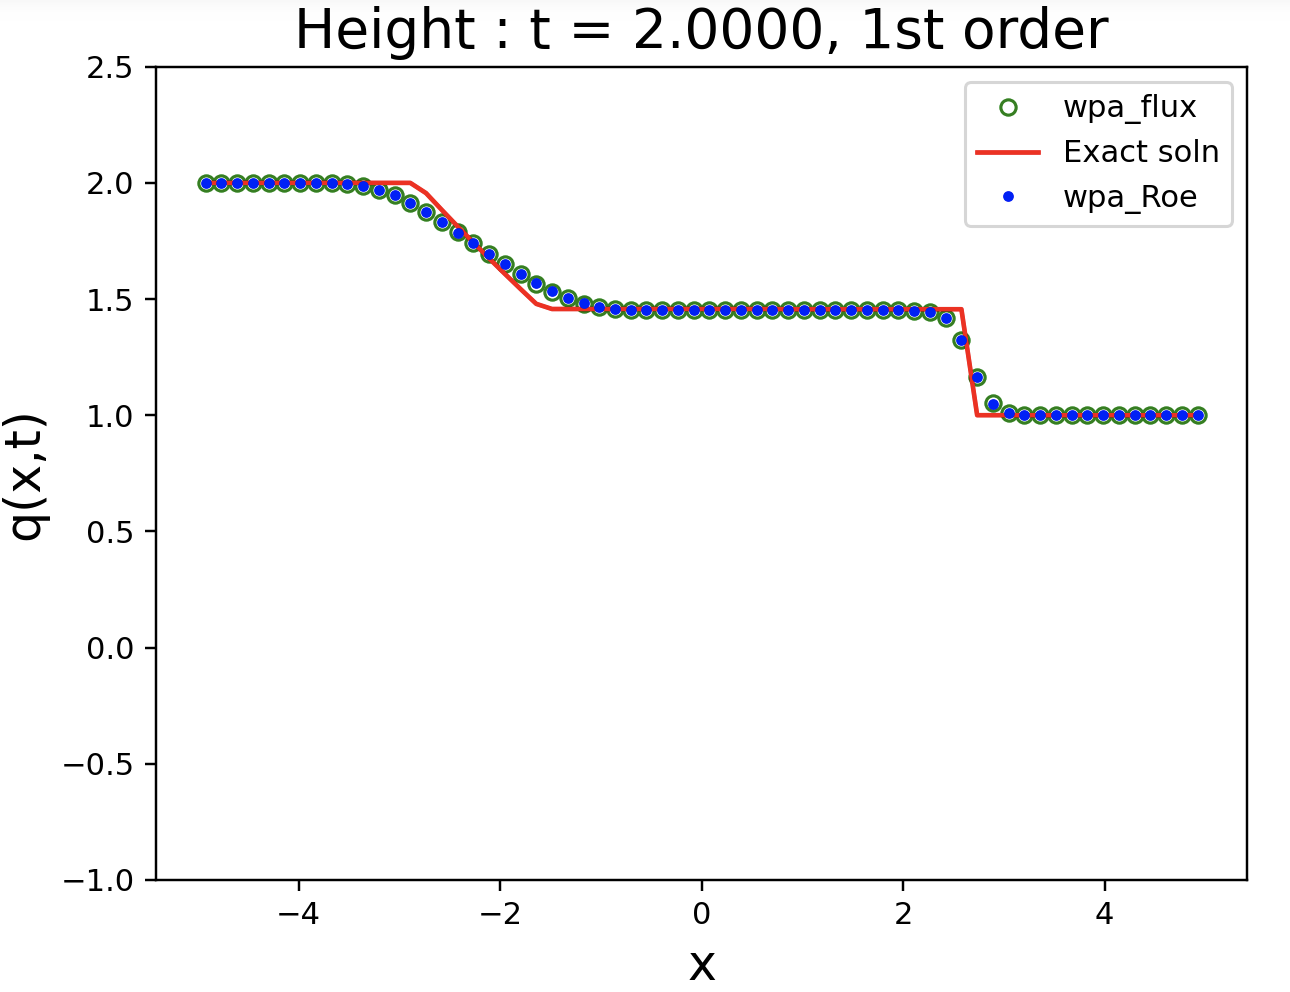
\includegraphics[width=1.0\linewidth]{images/1st}
			\caption{}
			\label{fig:1st}
		\end{subfigure}
		%
		\begin{subfigure}[b]{0.5\textwidth}
			\centering
			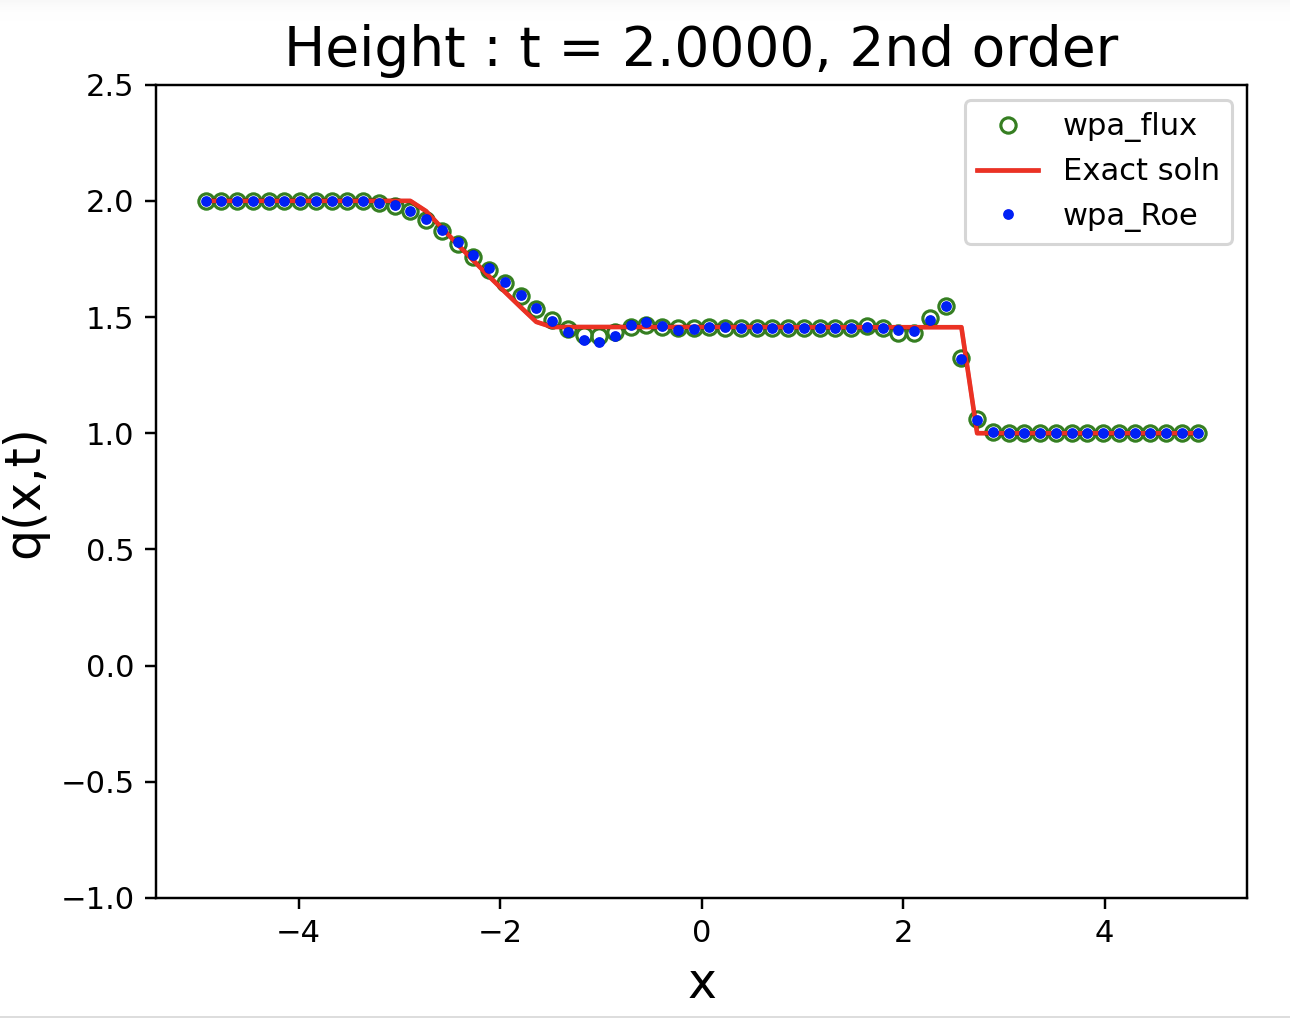
\includegraphics[width=1.0\linewidth]{images/2nd}
			\caption{}
			\label{fig:2nd}
		\end{subfigure}
		\caption{(a) and (b) respectively show height field at the final time step for both first and second order correction without limiters using 64 space points. }
	\end{figure}

\noindent Figure.~\ref{fig:2lim} depicts the filteration of oscillations around the 1-rarefaction fan and 2-shock discontinuity regions in fig.~\ref{fig:2nd} after application of limiters at the final time. It's seen that the hieght field solution exhibits a smooth through out the the entire simulation even at jumps in the solution compared to  fig.~\ref{fig:2nd}. This improved the accuracy of the second order method, simulating well the boundaries of several regions without noise.
\begin{figure}[H]
	\centering
	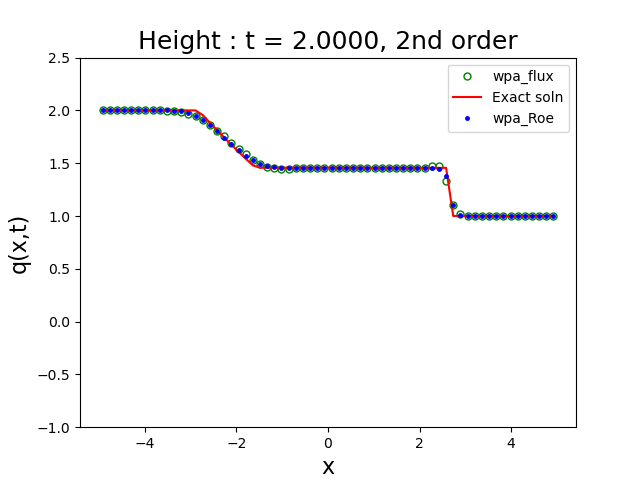
\includegraphics[width=0.85\linewidth]{images/2lim}
	\caption{Shows the height field at the final time step of second order correction with limiter uisng 64 space points.}
	\label{fig:2lim}
\end{figure}


	
	\subsection{ Bathymetric source terms}
	Equations \eqref{p1} and \eqref{p2}, can be extended to balance equations by introducing a bathymetric source term as shown in equations \eqref{bst} and  \eqref{bst0}. This is done by discretising the source term to generate values $-gh_{i-\frac{1}{2}}B^{\prime}(x_{i-\frac{1}{2}})$ at  cell interfaces  $x = x_{i-\frac{1}{2}}$. This approach is very useful, because the discrepancy caused due to the failure of the flux gradient to counterbalance the source term in a near steady state solution is decomposed into propagating waves  making the approach more robust than the quasi-steady WPA \cite{ba-le-mi-ro:2003}.
	\begin{eqnarray}
		h_{t} + (uh)_x &=& 0 
		\label{bst0}\\
		(hu)_t + \left(hu^{2} + \frac{1}{2}gh^{2} \right)_x &=& -ghB^{\prime}(x)
		\label{bst}
	\end{eqnarray}
	
	\noindent where $B(x)$ represents bottom elevation. \\
	
	%\subsection{ Introduce fwaves to handle stationery states}
	\noindent The fwaves are introduced to handle the stationery states and also solve accurately  the quasi-steady problems in which the objective is to obtain propagation due to small amplitude pertubations. The standard WPA (\ref{section:my}) is conservative if and only if equation \eqref{con} is satisfied, but the flux-based wave decomposition yields a more flexible algorithm that is conservative even when equation\eqref{con} is not satisfied. And works perfect even for problems in which the Roe average is not easily computed \cite{ba-le-mi-ro:2003}.
	
	\begin{equation}
		A_{i-\frac{1}{2}} (Q_{i} - Q_{i-1}) = f(Q_i) - f(Q_{i-1})
		\label{con}
	\end{equation}
	
	\noindent The flux difference $ f(Q_i) - f(Q_{i-1})$ is directly decomposed as  a linear combination of the eigen vectors $r_{i-\frac{1}{2}}$ as shown in equation \eqref{fw}
	
	\begin{equation}
	f(Q_{i}) - f(Q_{i-1})  - \Delta x \psi_{i-\frac{1}{2}} = \sum_{p=1}^{m} \beta_{i-\frac{1}{2}} ^{p} r_{i-\frac{1}{2}}^{p}  \equiv \sum_{p=1}^{m} \mathcal{Z}_{i-\frac{1}{2}}^{p} 
	\label{fw}
	\end{equation}
	where
	
	\begin{equation}
		\beta_{i-\frac{1}{2}} = R_{i-\frac{1}{2}}^{-1} (f(Q_{i}) - f(Q_{i-1}))  - \Delta x \psi_{i-\frac{1}{2}}
		\label{fw1}
	\end{equation}
	
	\noindent The vectors $\mathcal{Z}^{p} = \beta^{p} r^p$ are called the fwaves, as they are similar to the waves $\mathcal{W}^p$ though they carry flux increments rather than $q$ increments. The standard WPA (\ref{section:my}) first and second order corrections have been advanced to capture the flux based wave decompostion by changing equations \eqref{wpa19} and  \eqref{wpa13}  to  \eqref{fw1} and \eqref{fw2} respectively.
	
		\begin{equation}
		\tilde{F}_{i-\frac{1}{2}}^{n} = \frac{1}{2} \sum_{p=1}^{m}  \text{sgn}(s_{i- \frac{1}{2}}^{p}) \left( 1 - \frac{\Delta t}{\Delta x} |s_{i- \frac{1}{2}}^{p}|\right) \tilde{\mathcal{Z}}_{i-\frac{1}{2}}^{p} 
		\label{fw2}
	\end{equation}
	
	\noindent where $ \tilde{\mathcal{Z}}_{i-\frac{1}{2}}^{p} $ is also a limited version of the f-wave $ \mathcal{Z}_{i-\frac{1}{2}}^{p} $, obtained in the same way as $ \tilde{\mathcal{W}}_{i-\frac{1}{2}}^{p}$ was obtained from $ \mathcal{W}_{i-\frac{1}{2}}^{p}$. As seen in fig.\ref{fig:f2}, the second order correction term for the f-wave approach(wpa\textunderscore flux) phased out the oscillations near discontinouities without employing any limiter compared to the Roe-solver that employed the standard WPA. This means that the statinery waves near the discontinouities have been handled by the f-wave approach.\\
	
	\noindent Figures.~\ref{fig:f1} and \ref{fig:f2}, depicts the first and second order correction of the flux base wave decomposition(green), exact Riemann solution(red), and Roe-solver(blue) based on the standard WPA for the dambreak problem height field simulated at the final time without limiters. Fig.~\ref{fig:f1}  shows that both solutions concide, but the difference is exbited in the \ref{fig:f2} in which the Roe solver is highly affected by the oscillations near discontinouities in absence of limiters. This basically means that the f-wave approach together with the flux term filtered out the oscilliatory terms.

	\begin{figure}[H]
		\begin{subfigure}[b]{0.5\textwidth}
			\centering
			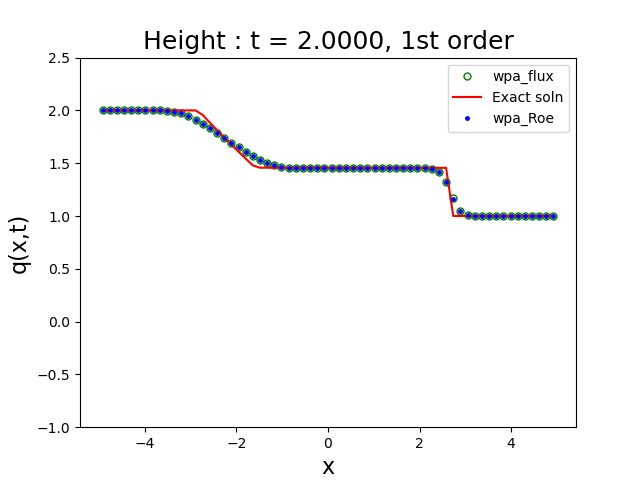
\includegraphics[width=1.0\linewidth]{images/f1}
			\caption{}
			\label{fig:f1}
		\end{subfigure}
		%
		\begin{subfigure}[b]{0.5\textwidth}
			\centering
			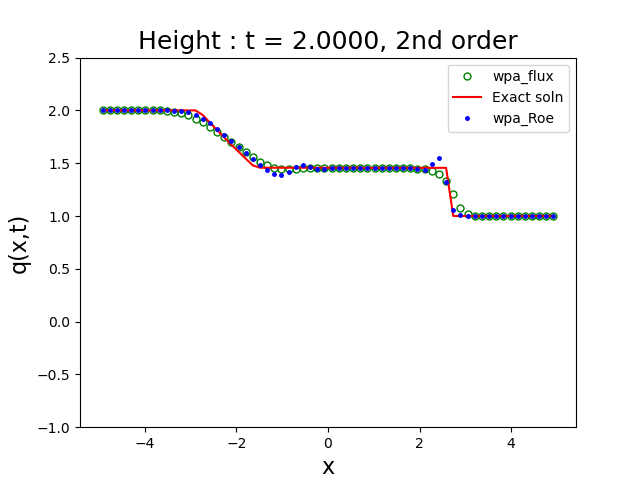
\includegraphics[width=1.0\linewidth]{images/f2}
			\caption{}
			\label{fig:f2}
		\end{subfigure}
		\caption{(a) and (b) respectively show height field at the final time step for both first and second order correction without limiters obtained after introducing the source term and the f-wave method. }
	\end{figure}
	
	\noindent Figure.~\ref{fig:f2lim} represents Figure.~\ref{fig:f2}  with limiters used. THe limiters made the Roe solver solution non osillatory(smooth through out), and rectified the solution of the f-wave approach to replicate the jump at the 2-shock but no stationary wave was present in the solution.
\begin{figure}[H]
	\centering
	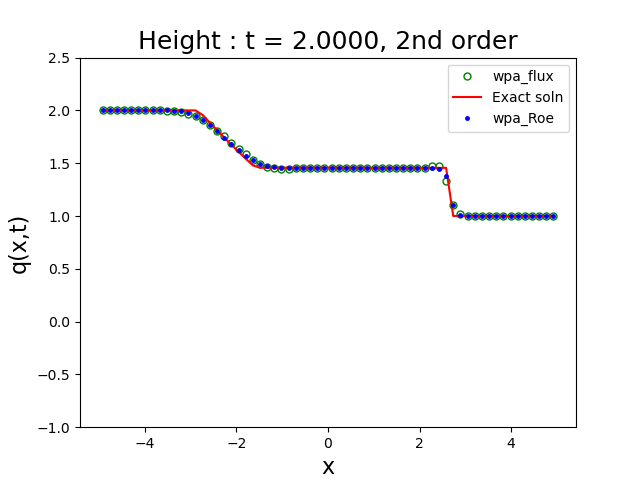
\includegraphics[width=0.85\linewidth]{images/2lim}
	\caption{Shows the height field at the final time step of second order correction with limiter obtained after introducing the source term and the f-wave method uisng 64 space points.}
	\label{fig:f2lim}
\end{figure}
	\section{Reimann Problem for Wet/Dry States}
	
	Dry states are regions with zero water depth. In such states SWEs are not applicable, so we consider wet states adjacent to dry regions as shown in figure~\ref{fig:dry-bed}. This enables solving SWEs in wet states, right up the boundary between wet and dry states \citep{toro2001shock}.
	\begin{figure}[H]
		\centering
		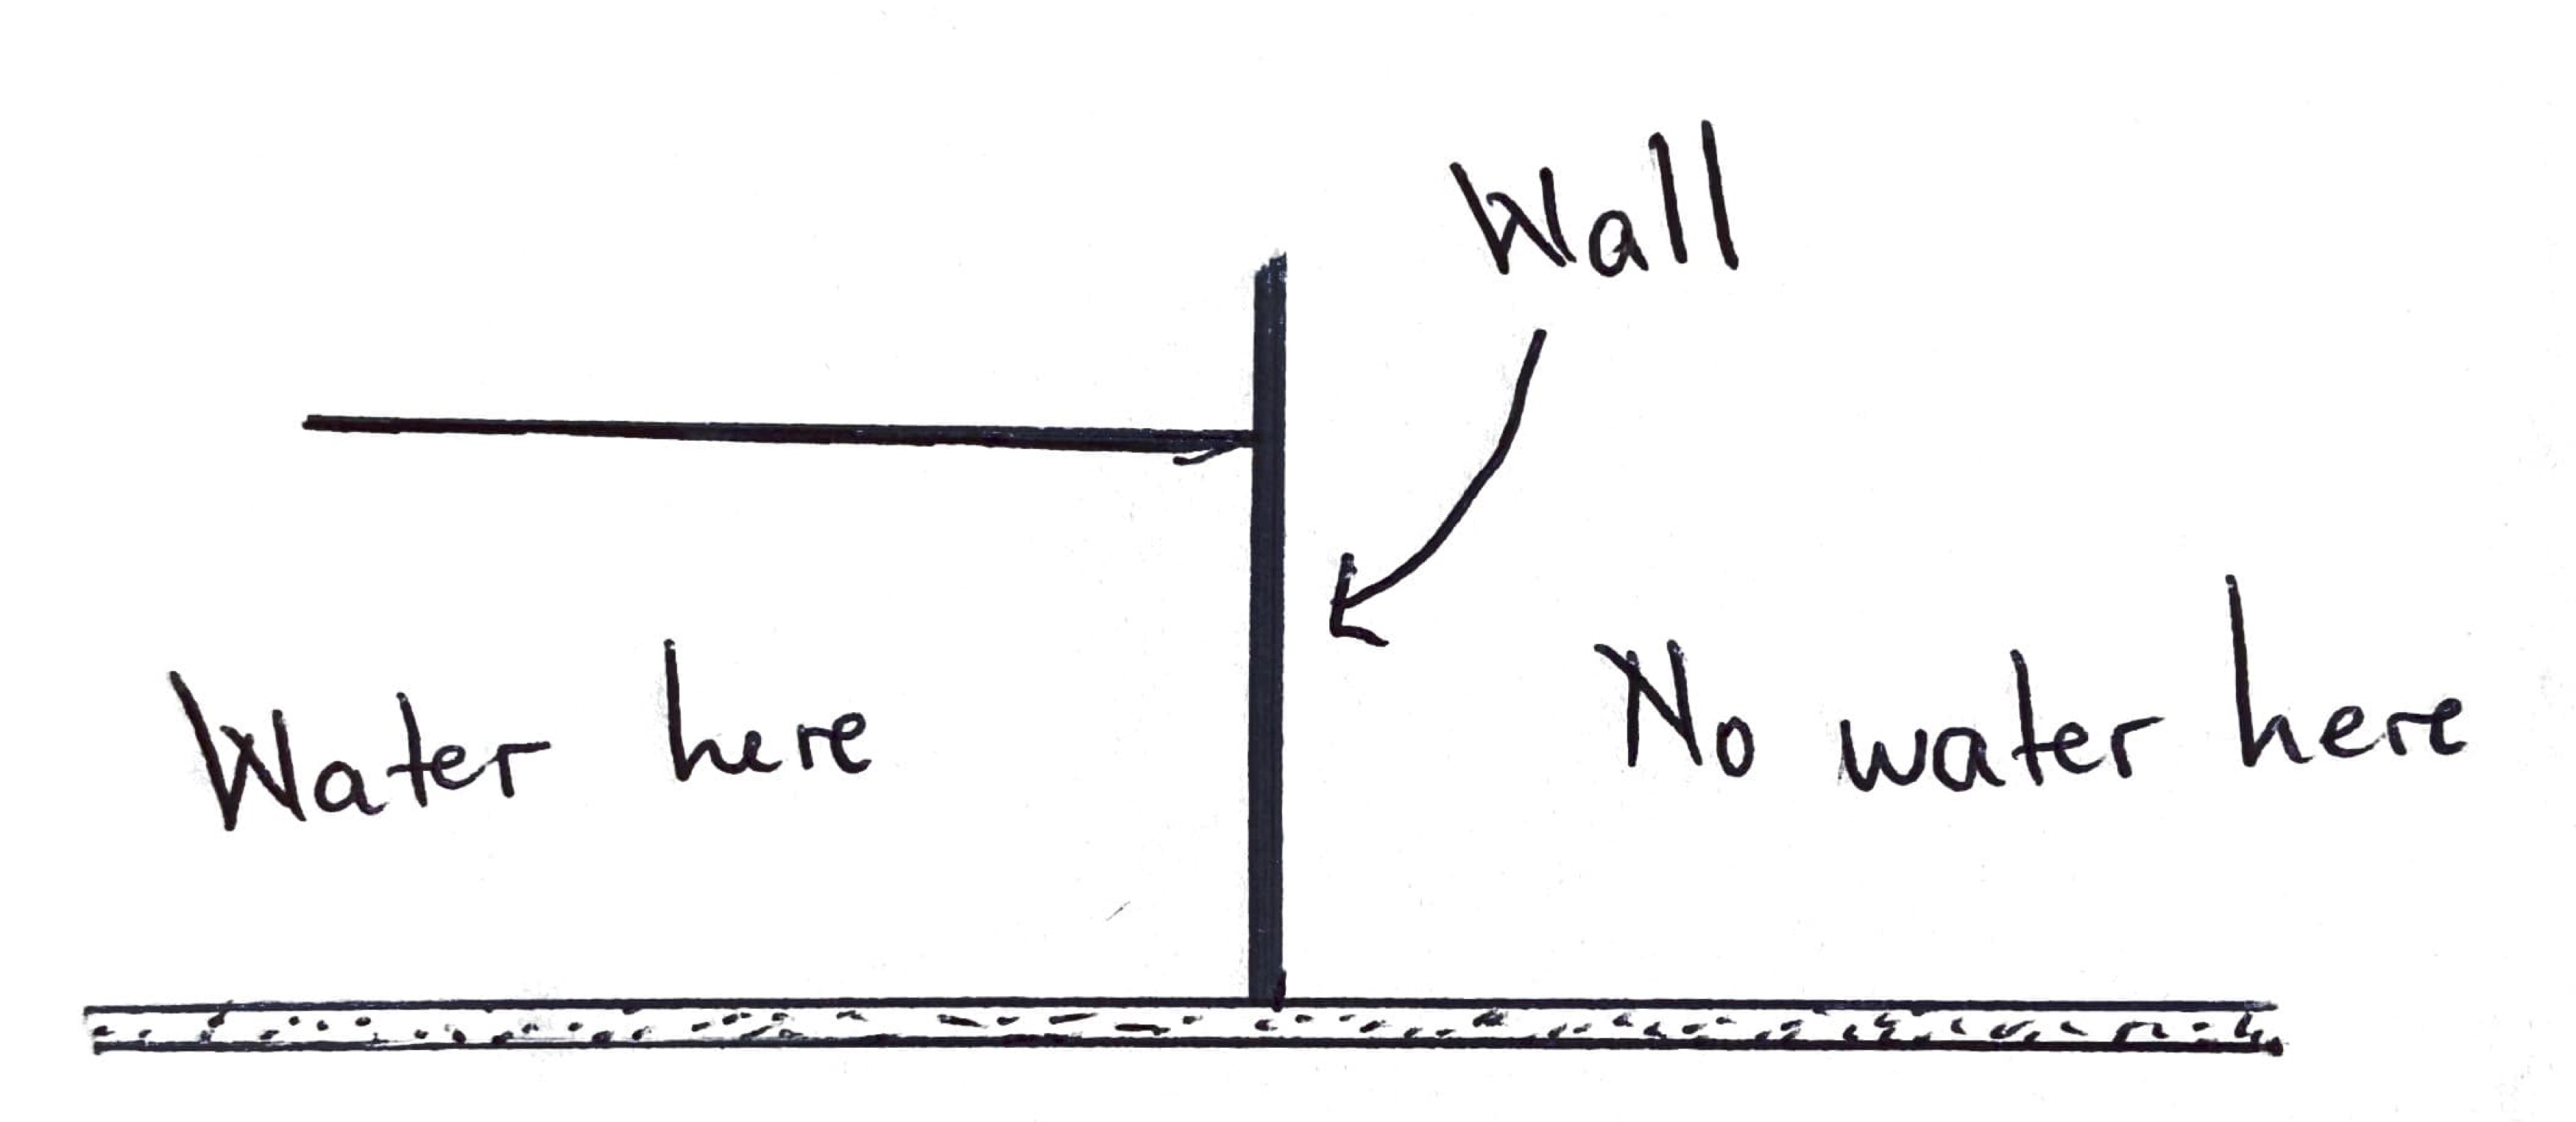
\includegraphics[width=0.7\linewidth]{images/db}
		\caption{ The Riemann problem with a dry bed (has no water) in one of the data state.}
		\label{fig:dry-bed}
	\end{figure}
	
	\noindent There is only one rarefaction in the exact Riemann solution, that connects wet to dry state. The developing wet/dry interface is in this case single edge of the rarefaction, making it possible to determine the interface propagating speed using the corresponding characteristics field of the Riemann invariants \cite{ge:2008}.\\ 
	
	\noindent The wet/dry interface propagation  speed  is given by equation \eqref{wd0}, since the right state in figure \ref{fig:dry-bed}, is considered as the initial dry state, which also makes the rarefaction to be in the first characteristic field.
	
	\begin{equation}
		s_{i-\frac{1}{2}}^{3} = \check{s}_{i-\frac{1}{2}}^{+} = \lambda_{i-\frac{1}{2}}^{-*}(0)= U_{i-1} - 2\sqrt{gH_{i-1}}
		\label{wd0}
	\end{equation}
	
	\noindent If the left state in figure \ref{fig:dry-bed}, is considered as the initial dry state, then the  wet/dry interface propagation  speed  is given by equation \eqref{wd0}, and the  rarefaction is in the second characteristic field .
	
\section{ Future research directions}
	
	
	
	
	
	\bibliographystyle{plain}
	\bibliography{geoclaw}
	
\end{document}

